%\newpage
\section{Измерение полупроводниковых элементов}
Исследование элемента необходимо начинать с обесточенным управляющим
выводом (третий вывод, назван TriStatePin). TriStatePin исследуемого
элемента во время испытания является  базовым или отправным. Один
испытательный вывод выбран положительной стороной элемента и
подключен непосредственно к VCC. Другой испытательный вывод выбран
отрицательной стороной элемента.
Отрицательная сторона подсоединена через резистор \(680~\Omega\) к GND.
Состояние полевых транзисторов зависит
от напряжения на затворе. Сначала, TriStatePin на \(5~ms\) подключается
через резистор \(680~\Omega\) Ом к GND и измеряется напряжение на отрицательной
стороне. Далее TriStatePin переключается на Ввод (высокое полное
входное сопротивление) и снова измеряется напряжение отрицательного
испытательного вывода. Затем предполагаемый затвор соединяется через
резистор \(680~\Omega\) на \(5~ms\) к VCC и снова измеряется напряжение на
отрицательной  стороне. Если измеренное напряжение ниже первого
результата измерения, то эта схема будет предполагаться, как
правильная. Затем напряжение снова измеряется с обесточенным TriStatePin.\\

Если напряжение отрицательного испытательного вывода с фиксированным 
напряжением TriStatePin выше чем \(115~mV\), а с обесточенным TriStatePin 
не ниже \(100~mV\), предполагается, что это обеднённый транзистор.\\

У биполярных транзисторов, имеющих повышенный обратный ток коллектора,
он значительно повышается в режиме с обесточенной базой.\\

При проверке с обоими напряжениями можно избежать неправильного
обнаружения некоторых германиевых транзисторов с более высоким
обратным током коллектора, как обедненных транзисторов (JFET).\\

Далее проводятся дополнительные тесты по определению N-канального JFET
или N D-MOSFET и P-канального JFET или P-D MOSFET. Версии MOSFET
могут быть определены по отсутствующему току затвора при любом
состоянии TriStatePin.\\

Чтобы получить параметры FET обеднённого типа, их измеряют с резистором \(680~\Omega\) в истоке, 
как показано на рисунке~\ref{fig:JFETcd} . Это измерение делается вместо обычного измерения тока 
удерживания затвора на уровне истока, потому, что \(I_\mathrm{DSS}\) FET транзистора часто не может 
быть достигнуто из-за относительно высокого сопротивления резистора \(680~\Omega\).

\begin{figure}[H]
\centering
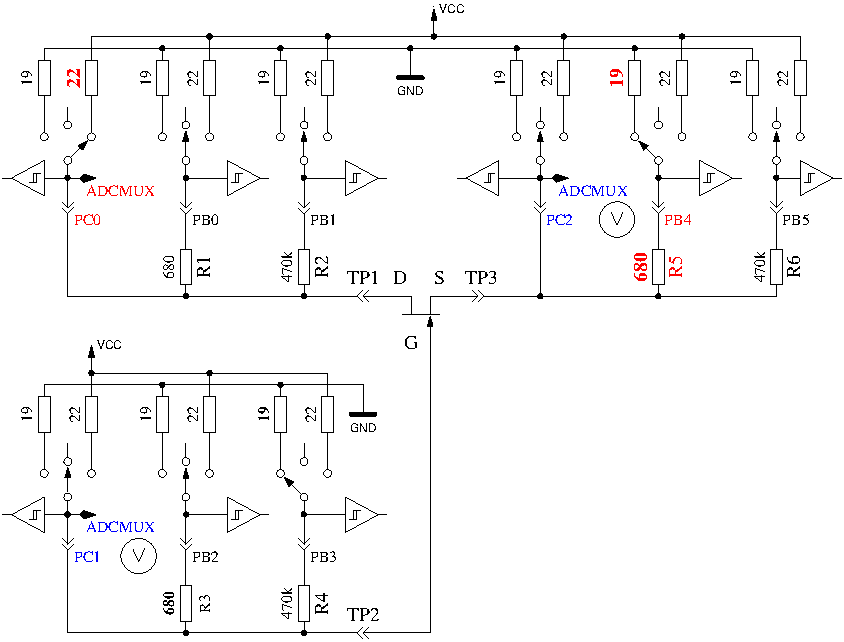
\includegraphics[width=.8\textwidth]{../FIG/JFETcd.pdf}
\caption{Измерение напряжения затвор-исток и тока истока N-JFET транзистора }
\label{fig:JFETcd}
\end{figure}

Если у элемента нет тока между положительным и отрицательным испытательными выводами без сигнала на TristatePin, 
то переходим к тестам определения, описанным в  разделе~\ref{sec:pnp}.
Если ток был обнаружен, то следующий тест описан в~\ref{sec:diode} о диодах.

\subsection{Измерение P-N-P транзистора или P-Channel-MOSFET}
\label{sec:pnp}
Сначала измеряют коэффициент усиления предполагаемого P-N-P транзистора в схеме с общим коллектором 
(эмиттерный повторитель). Схема измерения показана на рисунке~\ref{fig:pnpcc}.
Если напряжение базы (\(UB\)) измеренное с резистором \(680~\Omega\),  выше \(9~mV\), то коэффициент 
усиления вычисляется по формуле \(hFE = \frac{UE-UB}{UB}\).
Напряжение \(UE\) это разность между напряжением на эмиттере и VCC. Различие между резисторами \(22~\Omega\) 
и \(19~\Omega\) не учитывается. Если напряжение \(UB\) ниже \(10~mV\), измерение делают с резистором \(470~k\Omega\) 
в базе. В этом случае коэффициент  
усиления вычисляется по формуле \(hFE = \frac{UE \cdot 470000}{UB \cdot (680+22)}\).

\begin{figure}[H]
\centering
 \begin{overpic}[width=1.\textwidth]{../FIG/PNPcc.pdf}
  \color{black}
  \put(55,20){\makebox(0,0)[lb]{\footnotesize {\textcolor{green}{зеленым} switch state is used,}}}  
  \put(55,17){\makebox(0,0)[lb]{\footnotesize {if Voltage at PC1 is \textless~ 10mV!}}}      
 \end{overpic}
\caption{Измерение hFE P-N-P транзистора в схеме с общим коллектором }
\label{fig:pnpcc}
\end{figure}

Затем делают тесты для предполагаемого P-N-P транзистора в схеме с общим эмиттером. Положительная сторона 
элемента теперь подключена прямо с VCC, отрицательная сторона через резистор \(680~\Omega\) подключена к GND, 
как показано на рисунке~\ref{fig:pnpce}. 
Если на отрицательной стороне элемента есть напряжение выше \(3,4~V\), когда базовый резистор \(680~\Omega\) 
подключен к GND, значит этот элемент или P-N-P транзистор или P канальный FET. Какой из них - может быть легко 
установлено по напряжению базы. Если напряжение базы больше \(0,97~V\), это должен быть P-N-P транзистор. Для того, 
чтобы измерить коэффициент усиления, в цепь базы вместо резистора \(680~\Omega\) включается резистор \(470~k\Omega\).
Коэффициент усиления вычисляется по формуле \(hFE = \frac{(UC-UC0) \cdot 470000}{UB \cdot (680+19)}\) .
Напряжение UC0 является напряжением на коллекторном резисторе без базового тока. Как предполагается, правильным 
является более высокий коэффициент усиления, определенный первым или вторым способом. В версии 1.08k коэффициент 
усиления в схеме с общим эмиттером определяется только для микроконтроллеров ATmega328. Для других микроконтроллеров 
используется только схема с общим коллектором.\\

Значения, найденные для P-N-P транзистора, действительны только, если сделаны дополнительные измерения. Чтобы 
предотвратить обнаружение P-N-P транзистора в инверсном включении (коллектор с эмиттером поменяны местами), 
измерение с более высоким коэффициентом усиления считается правильным. 
Если напряжение базы ниже, чем \(0,97~V\), то это должен быть P-E-MOS. В этом случае пороговое напряжение затвора 
измеряется при плавном переключении затвора с резистором \(470~k\Omega\) от VCC до GND, ожидая на цифровом входе 
изменения  сигнала  стока, и затем, считывается напряжение затвора.

\begin{figure}[H]
\centering
 \begin{overpic}[width=1.\textwidth]{../FIG/PNPce.pdf}
  \color{black}
  \put(55,21){\makebox(0,0)[lb]{\footnotesize {The black state is used for Test!}}}  
  \put(55,17){\makebox(0,0)[lb]{\footnotesize {\textcolor{green}{зеленым} state is used for current}}} 
  \put(55,13){\makebox(0,0)[lb]{\footnotesize {gamplification factor hFE!}}}      
 \end{overpic}
\caption{Испытание и измерение hFE P-N-P транзистора в схеме с общим эмиттером }
\label{fig:pnpce}
\end{figure}

\subsection{Измерение N-P-N транзистора или N-Channel-MOSFET}
Измерение N-P-N транзистора начинается таким же образом, как и P-N-P транзистора, с измерения коэффициента усиления 
в схеме с общим коллектором.
Первое измерение сделано с резистором в цепи базы \(680~\Omega\) подключенным к VCC. Если напряжение на резисторе в 
цепи базы слишком низко, вместо \(680~\Omega\) берётся резистор \(470~k\Omega\).
Тогда измерение продолжается в схеме с общим эмиттером, как показано на рисунке~\ref{fig:npnce}.
Если напряжение коллектора ниже \(1,6~V\) и резистор в цепи базы \(680~\Omega\) соединён с VCC, то это может быть N-P-N 
транзистор, N-канальный MOSFET или тиристор/симистор. Тиристор или симистор могут быть идентифицированы двумя 
простыми тестами. Если резистор на управляющем выводе, соединённый в течение \(10~ms\) с GND обесточить, ток в аноде 
должен остаться. Если резистор анода кратковременно подключить к GND и, затем, повторно подключить к VCC, тиристор 
не должен снова включиться (нет тока). Имейте в виду, что Тестер может проверять только маломощные тиристоры, потому 
что ток удержания может достигать только \(6~mA\). Если оба теста свидетельствуют о тиристоре, то необходимо сделать 
тесты с обратной полярностью, чтобы исключить или подтвердить симистор. 
\begin{figure}[H]
\centering
 \begin{overpic}[width=1.\textwidth]{../FIG/NPNce.pdf}
  \color{black}
  \put(55,23){\makebox(0,0)[lb]{\footnotesize {The black state is used for Test!}}}  
  \put(55,19){\makebox(0,0)[lb]{\footnotesize {\textcolor{green}{зеленым} state is used for current}}} 
  \put(55,15){\makebox(0,0)[lb]{\footnotesize {amplification factor hFE!}}}      
 \end{overpic}
\caption{Испытание и измерение hFE N-P-N транзистора в схеме с общим эмиттером }
\label{fig:npnce}
\end{figure}
Если ни тиристор, ни симистор не были подтверждены, то это может быть N-P-N транзистор или N канальный E-MOSFET. 
Базовое напряжение N-P-N транзистора будет близко к напряжению эмиттера, таким образом, этот тип может быть 
идентифицирован определенно. Коэффициент усиления в схеме с общим эмиттером вычисляется по формуле 
\(hFE = \frac{(VCC-UC-UC0)\cdot 470000}{(VCC-UB)\cdot (680+22)}\).
Если напряжение базы или затвора повышенные, то в этой цепи тока нет или он мал, значит, элемент будет N-канальным  
E-MOS (MOSFET обогащённый). В этом случае пороговое напряжение измеряется при плавном переключении затвора с 
резистором \(470~k\Omega\) от VCC до GND, ожидая на цифровом входе изменения сигнала стока, и затем считывается 
напряжение затвора. Это измерение делается 11 раз с накоплением результатов АЦП, как показано на 
рисунке~\ref{fig:eleven}.
Результат умножается на 4 и делится на 9, чтобы получить напряжение в \(mV\).
\begin{figure}[H]
\centering
\includegraphics[width=.8\textwidth]{../PNG/IRFU120gate.png}
\caption{Измерение порогового напряжения N-канального MOSFET}
\label{fig:eleven}
\end{figure}

\subsection{Упрощенная блок-схема тестирования транзисторов}

\begin{figure}[H]
\centering
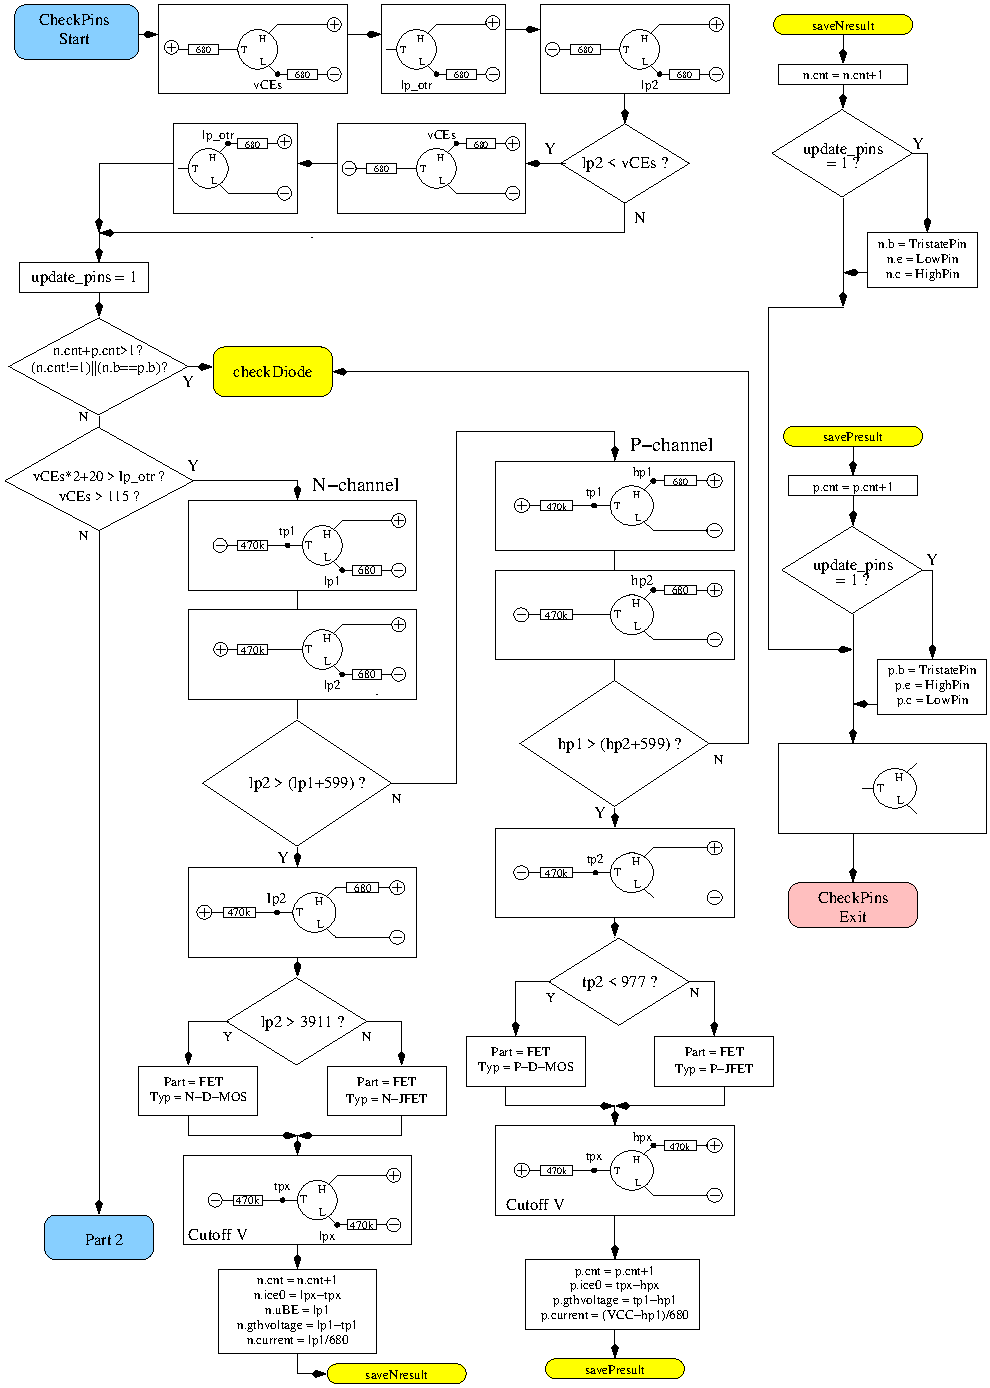
\includegraphics[width=.95\textwidth]{../FIG/CheckSemi1.pdf}
\caption{Блок-схема тестирования транзисторов. Часть 1: JFET и D-MOS}
\label{fig:ChkSemi1}
\end{figure}

\begin{figure}[H]
\centering
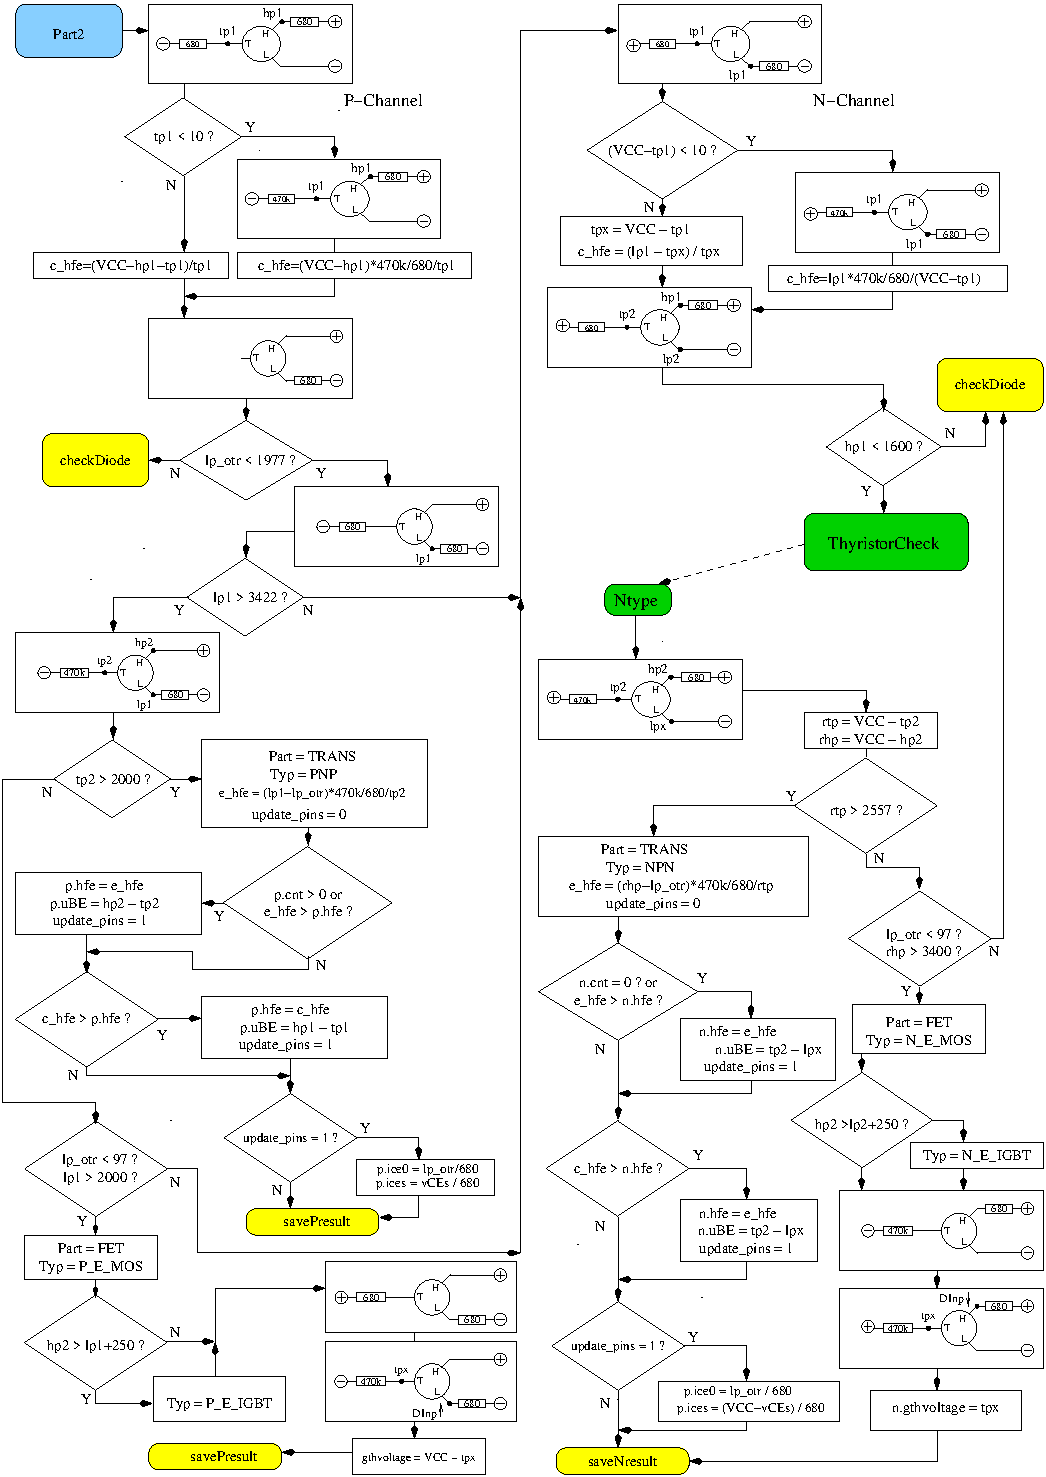
\includegraphics[width=.95\textwidth]{../FIG/CheckSemi2.pdf}
\caption{Блок-схема тестирования транзисторов. Часть 2: BJT и E-MOS}
\label{fig:ChkSemi2}
\end{figure}

\begin{figure}[H]
\centering
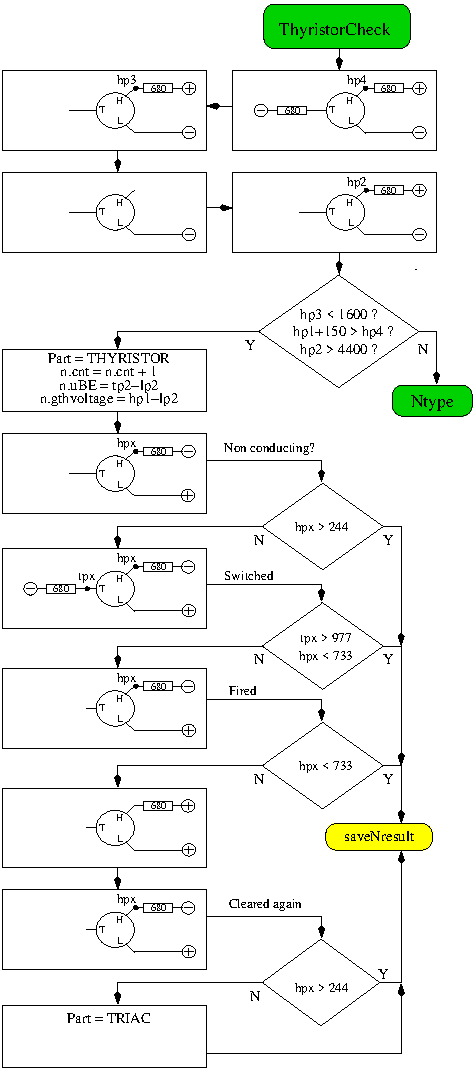
\includegraphics[width=.95\textwidth]{../FIG/CheckSemi3.pdf}
\caption{Блок-схема тестирования транзисторов. Часть 3: Тиристор и симистор}
\label{fig:ChkSemi3}
\end{figure}


\subsection{Измерение диодов}
\label{sec:diode}
Если предварительными тестами будет обнаружен ток, то элемент будет опознан как диод. Падение напряжения с 
резистором \(680~\Omega\) должно быть между \(0,15~V\) и \(4,64~V\). Падение   напряжения с резистором \(680~\Omega\) 
должно быть в 1.125 раза больше падения напряжение с резистором \(470~k\Omega\) и падение  напряжения с 
резистором \(470~k\Omega\) должно быть в 16 раз больше, 
чем падение  напряжения с резистором \(680~\Omega\). Дополнительно: при возобновлении измерения с 
резистором \(470~k\Omega\) напряжения должно быть не выше, чем в предыдущем измерении с 
резистором \(680~\Omega\).
Я надеюсь, что этот метод всегда идентифицирует диод. При идентификации двух диодов, включенных встречно-параллельно, 
невозможно определение тока утечки в противоположном направлении. Если обнаружен только одиночный диод, то ток 
утечки в обратном направлении измеряется с резистором \(470~k\Omega\) подключенным к VCC. Разрешение около \(2~nA\).
Если ток  утечки больше \(5,3~\mu A\) (напряжение на резисторе \(470~k\Omega\) составляет больше чем \(2,5~V\)), 
измерение производится с резистором \(680~\Omega\).
В этом случае разрешение только около \(1~\mu A\).
Кроме того, для одиночного диода, может быть измерена ёмкость в обратном направлении.

\subsection{Результаты различных измерений}
Следующие таблицы показывают результаты испытательных исследований с различными микроконтроллерами 
ATmega8, ATmega168, ATmega328.

\begin{table}[H]
  \begin{center}
    \begin{tabular}{| l | c | c | c |}
    \hline
   Тип диода & Mega8@8MHz & Mega168 @8MHz & Mega328 @8MHz \\                
    \hline
    \hline
1N4148     & Diode, 715mV,        & Diode, 718mV,            & Diode, 715mV,           \\
           &               1pF    &               0pF, 2nA   &               1pF, 4nA  \\
    \hline
1N4150     & Diode, 665mV,        & Diode, 672mV,            & Diode, 666V,           \\
           &               1pF    &               1pF, 4nA   &              2pF, 6nA  \\
    \hline
BA157      & Diode, 619mV,        & Diode, 621V,              & Diode, 615mV,            \\
           &               19pF   &              17pF, 12nA   &               18pF, 12nA \\
    \hline
BY398      & Diode, 538mV,        & Diode, 541mV,             & Diode, 537mV,            \\
           &               16pF   &               14pF, 63nA  &               15pF, 63nA \\
    \hline
1N4007     & Diode, 650mV,        & Diode, 655mV,            & Diode, 650mV,           \\
           &               13pF   &               10pF, 6nA  &               13pF, 6nA \\
    \hline
LED green  & Diode, 1,96V, 5pF    & Diode, 1,95V, 4pF   & Diode, 1.95V, 4pF \\
    \hline
ZPD2,7     & 2xDi, 743mV, 2,53V   & 2xDi, 737mV, 2,52V  & 2xDi, 733mV, 2,51V \\
    \hline
BU508A B+E & Diode, 609mV,        & Diode, 611mV,                & Diode, 606mV,              \\
           &               5,15nF &               5,20nF, 0,39uA &               5,25nF, 0,4uA\\
    \hline
BU508A B+C & Diode, 582mV,        & Diode, 586mV,             & Diode, 587mV,            \\
           &               256pF  &               255pF, 21nA &               259pF, 19nA\\
    \hline
AC128 B+E  & Diode, 272mV,        & Diode, 277mV,              & Diode, 273mV,             \\
           &               0pF    &               0pF, 2,2uA   &               0pF, 2,3uA  \\
    \hline
AC128 B+E  &                      &                     & Diode, 349mV,               \\
с охлаждением     &                      &                     &               140pF, 0,57uA \\
    \hline
MBR20100CT & 2xDi, 337mV, 337mV   & 2xDi, 338mV, 338mV  & 2xDi, 336mV, 335mV  \\
    \hline
MBR20100CT & Diode, 337mV,        & Diode, 339mV,             & Diode, 337mV,            \\
           &               345pF  &               351pF, 29nA &               350pF, 25nA\\
    \hline
MBR4045PT  & Diode, 243mV,        & Diode, 233mV,               & Diode, 235mV,              \\
с охлаждением     &               1,80nF &               1,94nF, 1,7uA &               1,95nF, 1,8uA\\
    \hline
SK14       & Diode,    mV,        & Diode,    mV,               & Diode, 263mV,              \\
           &                  0pF &                   pF,    nA &               0pF, 0,57uA\\
    \hline
SK14       & Diode,    mV,        & Diode,    mV,               & Diode, 334mV,              \\
с охлаждением     &                   nF &                   pF,    nA &               88pF, 4nA\\
    \hline
SF38G      & Diode, 519mV,        & Diode, 521mV,            & Diode, 516mV,            \\
           &               107pF  &               105pF, 2nA &               106pF, 2nA \\
    \hline
    \end{tabular}
  \end{center}
  \caption{Результаты измерения диодов}
  \label{tab:diodes} 
\end{table}

Измерение обратной ёмкости для двойного диода MBR4045PT возможно только с охлаждением. 
Это вызвано высоким током утечки этого \(40~A\) диода. Также обратная ёмкость перехода база-эмиттер 
германиевого транзистора AC128 может быть измерена только с охлаждением.

\begin{table}[H]
  \begin{center}
    \begin{tabular}{| l | c | c | c | c | c |}
    \hline
             Тип & Тип & Mega8           & Mega328        & Mega328         & Mega328 \\
Транзистора     & пр-ти     & общий         &                & общий         & общий \\
            &     & коллектор      &                & коллектор       & эмиттер \\
    \hline
    \hline
BU508A      & NPN & \(\beta\)=9, 601mV      &  \(\beta\)=9, 597mV    &   \(\beta\)=9, 598mV    & \(\beta\)=4, 484mV \\
    \hline
2N3055      & NPN & \(\beta\)=20, 557mV     &  \(\beta\)=21, 550mV   &   \(\beta\)=21, 550mV   & \(\beta\)=6, 442mV \\
    \hline
BC639       & NPN & \(\beta\)=148, 636mV    &  \(\beta\)=172, 629mV  &   \(\beta\)=172, 629mV  & \(\beta\)=158, 605mV \\
    \hline
BC640       & PNP & \(\beta\)=226, 650mV    &  \(\beta\)=176, 609mV  &   \(\beta\)=171, 655mV  & \(\beta\)=177, 608mV \\
    \hline
BC517       & NPN & \(\beta\)=23,9k, 1,23V  &  \(\beta\)=24,8k, 1,22V&   \(\beta\)=25,1k, 1,22V & \(\beta\)=764, 1,23V \\
    \hline
BC516       & PNP & \(\beta\)=75,9k, 1,21V  &  \(\beta\)=76,2k, 1,20V&   \(\beta\)=76,2k, 1,20V & \(\beta\)=760, 1,23V \\
    \hline
BC546B      & NPN & \(\beta\)=285, 694mV    &  \(\beta\)=427, 687mV  &   \(\beta\)=427, 687mV   & \(\beta\)=369, 683mV \\
    \hline
BC556B      & PNP & \(\beta\)=304, 704mV    &  \(\beta\)=254, 668mV  &   \(\beta\)=235, 709mV   & \(\beta\)=255, 668mV \\
    \hline
AC128 (Ge.) & PNP & \(\beta\)=63, 191mV     &  \(\beta\)=59, 191mV   &   \(\beta\)=57, 193mV    & \(\beta\)=43, 117mV \\
    \hline
BUL38D      & NPNp & \(\beta\)=37, 627mV    &  \(\beta\)=41, 617mV  &   \(\beta\)=40, 624mV     & \(\beta\)=36, 562mV \\
parasitic   & PNPn & \(\beta\)=11, 654mV    &  \(\beta\)=81, 543mV  &   \(\beta\)=10, 656mV     & \(\beta\)=83, 541mV \\
    \hline
BRY55/200   & Thyrist. &  0,84V     &  0,81V         &   0,81V          &  0,82V \\
    \hline
MAC97A6     & Triac    &  0,92V     &  0,90V         &   0,90V          &  0,90V \\
    \hline
    \end{tabular}
  \end{center}
  \caption{Результаты измерения биполярных транзисторов}
  \label{tab:bipolar} 
\end{table}

Некоторые результаты значительно отличаются от результатов, полученных в более ранних версиях программного 
обеспечения от Markus F. Например, транзистор Дарлингтона BC517 был измерен более ранним программным 
обеспечением: hFE=797 вместо 77200 и напряжение база-эмиттер = \(1438~mV\). Это вызвано дополнительным измерением 
коэффициента усиления в схеме с общим коллектором. Кроме того, новая версия программного обеспечения показывает 
такой же низкий результат hFE в схеме с общим эмиттером, что можно увидеть в последнем столбце 
таблицы~\ref{tab:bipolar}.
Напряжение база-эмиттер измерено как отдельный диод. Теперь напряжение база-эмиттер измеряется при токе измерения 
коэффициента усиления (\(1,20~V\)). NPN-транзистор BUL38D имеет между коллектором и эмиттером встроенный защитный диод, 
который может спровоцировать определение паразитного PNP-транзистора с базой на месте коллектора правильного 
NPN транзистора. С версии программного обеспечения 1.10k оба транзистора обнаруживаются и помечаются добавлением 
символа р. Правильный транзистор будет найден при сравнении ёмкости перехода база - эмиттер. Предполагается, 
что правильный транзистор имеет более высокую ёмкость перехода. Если нажать и удерживать клавишу запуска во время 
вывода результата измерения, то будут показаны параметры паразитного транзистора. Наличие правильного транзистора 
будет отмечено индексом n (PNPn). Паразитный транзистор определяется только с защитным диодом, расположенном на 
том же кристалле, что и правильный транзистор, а не с внешним диодом.\\

Следующая таблица~\ref{tab:germanium} показывает результаты измерения для германиевых транзисторов, которые являются 
проблемными из-за температурной зависимости и высокого обратного тока коллектора. Представлены вместе результаты 
оригинальной версии от Markus F. и результаты версии 1.10k. Версия 1.10k для ATmega328 измеряет коэффициент усиления 
в схемах с общим коллектором и общим эмиттером с учетом обратного тока коллектора, и выводит более высокий результат. 
Обратный ток коллектора не учитывался в более ранних версиях программного обеспечения.

\begin{table}[H]
  \begin{center}
    \begin{tabular}{| l | c | c | c |}
    \hline
      Тип & Mega8@1MHz          & Mega168 @8MHz       & Mega328 @8MHz    \\
 транзистора    & Оригинальная вер.    & Версия 1.10k       & Версия 1.10k  \\
            & Markus F.           &                     &        \\
    \hline
    \hline
AC128       & PNP, \(\beta\)=52, 279mV    & PNP, \(\beta\)=59, 184mV    & PNP, \(\beta\)=59, 191mV    \\
    \hline
AC116-65    & PNP, \(\beta\)=505, 378mV   & PNP, \(\beta\)=72, 146mV    & PNP, \(\beta\)=72, 149mV    \\
    \hline
AC116-145   & PNP, \(\beta\)=485, 294mV   & PNP, \(\beta\)=146, 161mV    & PNP, \(\beta\)=146, 163mV   \\
    \hline
AC176-65    & NPN, \(\beta\)=98, 235mV    & NPN, \(\beta\)=58, 94mV    & NPN, \(\beta\)=56, 96mV     \\
    \hline
GC122       & PNP, \(\beta\)=84, 368mV    & PNP, \(\beta\)=55, 117mV    & PNP, \(\beta\)=56, 117mV    \\
    \hline
GC301       & PNP, \(\beta\)=48, 289mV    & PNP, \(\beta\)=39, 184mV    & PNP, \(\beta\)=39, 188mV    \\
    \hline
AD161       & NPN, \(\beta\)=360, 230mV   & NPN, \(\beta\)=296, 126mV   & NPN, \(\beta\)=298, 128mV    \\
    \hline
AD162       & PNP, \(\beta\)=2127, 280mV  & PNP, \(\beta\)=89, 107mV    & PNP, \(\beta\)=89, 107mV    \\
    \hline
    \end{tabular}
  \end{center}
  \caption{Результаты измерений германиевых биполярных транзисторов}
  \label{tab:germanium}
\end{table}

В таблице~\ref{tab:mos} показаны результаты измерения некоторых полевых транзисторов. Одним из измеряемых параметров 
E-MOS транзисторов является напряжение затвор-исток, которое замеряется по изменению состояния цифрового входа ATmega, 
подключенному 
к стоку через резистор \(680~\Omega\).
Из-за небольшой ёмкости затвора, напряжение на нем изменяется
очень быстро, что уменьшает точность фиксации этого напряжения. Например, у транзистора BS250 это напряжение
изменялось от \(2,6~V\) до \(2,5~V\), при подключении дополнительного конденсатора ёмкостью
\(10~nF\) параллельно выводам затвор и исток.
Другим измеренным параметром является значение ёмкости затвора.
Емкость затвора измеряется путем переключения вывода истока и затвора на GND.
Доступное напряжение \(5~V\) на затворе тестера является недостаточным для генерации достаточного тока
для некоторых IGBT. Это мешает правильному обнаружению.
В большинстве случаев обнаруживается только защитный диод коллектор-эмиттер.
Источник, примерно, \(3~V\), подключенный к выходу, может решить проблему с обнаружением.
Другой полюс источника должен быть подключен к тестовому выводу (TP) тестера вместо соединения затвора.
При правильной полярности батареи тестер должен обнаружить IGBT.
Отображаемое напряжение переключения затвор-сток должно быть увеличено на величину напряжения батареи,
чтобы получить правильное напряжение переключения.
Для JFET транзисторов в качестве характеристики часто приведен ток Idss,
являющийся током стока при напряжении затвор-исток равном \(0~V\). В данной реализации, однако, ток не может
превышать величины, определенной сопротивлением нагрузки в стоке JFET величиной \(680~\Omega\).
Нагрузочный резистор генерирует обратное напряжение Vgs, которое также отображается на индикаторе.
С нагрузочным резистором \(470~k\Omega\) в цепи истока JFET ток исток-сток будет почти нулевым.
Таким образом, напряжение отсечки Vgs\_off исток-затвор может быть определено достаточно точно,
при условии, что оно не превысит \(5~V\).
С этими двумя рабочими точками мы можем определить ток затвор-исток Igss с почти среднеквадратичной точностью.
Если расчетный ток меньше \(40~mA\), дополнительно проводится измерение без сопротивления в цепи истока.
По более высокому напряжению на выводе истока без резистора мы можем вычислить дополнительное значение тока.
Используя эти результаты измерений, снова вычисляем ток затвор-исток Idss,
при этом он не должен превысить значения \(40~mA\).
Из-за симметричной конструкции транзисторов JFET, невозможно отличить сток от истока.


\begin{table}[H]
  \begin{center}
    \begin{tabular}{| l | c | c | c | c |}
    \hline
 Транзистор  &  Тип    & Mega8@8MHz       & Mega168 @8MHz    & Mega328 @8MHz \\
             &         &                  &                  &               \\
    \hline
    \hline
ZVNL120A     & N-E-MOS & D, 1,6V, 147pF   & D, 1,5V,141pF    & D, 1,5V, 140pF \\
    \hline
IRF530N      & N-E-MOS & D, 3,6V, 1.55nF  & D, 3,6V, 1,54nF  & D, 3,6V, 1,54nF \\
    \hline
BS170        & N-E-MOS & D, 2,6V, 78pF    & D, 2,6V, 68pF    & D, 2,6V, 68pF \\
    \hline
IRL3803      & N-E-MOS & D, 2,3V, 9.81nF  & D, 2,3V, 9,71nF  & D, 2,3V, 9,74nF \\
    \hline
IRFU120N     & N-E-MOS & D, 4,2V, 909pF   & D, 4,2V, 913pF   & D, 4,2V, 911pF \\
    \hline
BUZ71A       & N-E-MOS & D, 3,2V, 714pF   & D, 3,2V, 708pF   & D, 3,2V, 705pF \\
    \hline
ZVP2106A     & P-E-MOS & D, 3,2V, 122pF   & D, 3,2V,115pF    & D, 3,2V, 116pF \\
    \hline
IRF5305      & P-E-MOS & D, 3,6V, 2.22nF  & D, 3,6V, 2,22nF  & D, 3,6V, 2,22nF \\
    \hline
BS250        & P-E-MOS & D, 2,6V, 53pF    & D, 2,6V, 43pF    & D, 2,6V, 44pF \\
    \hline
IRFU9024     & P-E-MOS & D, 3,5V, 937pF   & D, 3,6V, 945pF   & D, 3,5V, 933pF \\
    \hline
J310         & N-JFET  & 3.1mA Vgs=2.2V   & 3.1mA Vgs=2.2V   & 3.1mA Vgs=2.2V \\
Idss=24-60mA &         &                  &                  & Idss=35mA      \\
    \hline
2N5459       & N-JFET  & 2.1mA Vgs=1.5V   & 2.1mA Vgs=1.5V   & 2.1mA Vgs=1.5V \\
Idss=4-16mA &          &                  &                  & Idss=8.2mA     \\
    \hline
BF256C       & N-JFET  & 3.4mA Vgs=2.4V   & 3.4mA Vgs=2.4V   & 3.4mA Vgs=2.4V \\
Idss=11-18mA &         &                  &                  & Idss=14mA      \\
    \hline
BF245A       & N-JFET  & 1.1mA Vgs=.75V   & 1.1mA Vgs=0.75V  & 1.1mA Vgs=0.75V \\
Idss=2-6mA   &         &                  &                  & Idss=3.6mA      \\
    \hline
BF245B       & N-JFET  & 2.5mA Vgs=1.7V   & 2.5mA Vgs=1.7V   & 2.5mA Vgs=1.7V \\
Idss=6-15mA  &         &                  &                  & Idss=10mA      \\
    \hline
BF245C       & N-JFET  & 3.9mA Vgs=2.7V   & 3.9mA Vgs=2.7V   & 3.9mA Vgs=2.7V \\
Idss=12-25mA &         &                  &                  & Idss=17mA    \\
    \hline
J175        & P-JFET   & 3.2mA Vgs=2.2V   & 3.2mA Vgs=2.2V   & 3.2mA Vgs=2.2V \\
Idss=7-60mA &          &                  &                  & Idss=26mA      \\
    \hline
2N5460      & P-JFET   & 0.78mA Vgs=0.54V & 0.77mA Vgs=0.54V & 0.78mA Vgs=0.54V \\
Idss=1-5mA  &          &                  &                  & Idss=2.6mA       \\
    \hline
BSS169      & N-D-MOS   & 2,6mA Vgs=1,8V & D, 2,6mA Vgs=1,8V & D, 2,6mA Vgs=1,8V \\
    \hline
GP07N120    & N-E-IGBT & C=3,81nF Vt=4,2V & C=3,76nF Vt=4,2V & C=3,74nF Vt=4,2V \\
    \hline
G4PC30      & N-E-IGBT &                  &                  & C=2.22nF         \\
с батареей  &          &                  &                  & Vt=2.0V+3.2V \\
    \hline
    \end{tabular}
  \end{center}
  \caption{Результаты измерений МОП-транзисторов}
  \label{tab:mos} 
\end{table}
